\renewcommand{\baselinestretch}{2} \small\normalsize
\chapter{Environmental Impacts on Electromagnetic Wave Propagation}
There are several environmental factors that can cause affect propagation. Multipath, clutter, and sea spikes are all induced by reflections from the sea surface while changes in the index of refraction can cause the electromagnetic waves to bend. 

\section{Earth Models}
The earth can be modeled as flat to simplify calculations, as a sphere to capture horizon effects for long range propagation, or as an ellipsoid as described in the WGS-84 model to provide additional geometric accuracy.

\subsection{Flat Earth}
The flat earth model is valid only for short ranges as there is no concept of the RADAR horizon.

TBD - add image

\subsection{Spherical Earth}
The spherical earth model assumes the earth is a sphere, with a constant radius $r_e = 6,370,000 m$.
TBD - add image

\subsection{WGS-84 Earth}
TBD - add discussion, image

\subsection{4/3 Earth Model}
Due to the refractive index of the atmosphere, the propagation path of an electromagnetic wave will curve. Under the assumption of standard atmospheric conditions, the propagation path can be approximated as a straight line if an effective radius of the earth is used $r_e' = 4/3 r_e$. This is referred to as the 4/3 earth model \cite{blake_radar} and is used in most analytical calculations.

\section{Geometry}
\subsection{Grazing and Depression Angles}
\subsection{RADAR Horizon}

\section{Atmospheric Refraction Effects}
\subsection{Refractivity}

\subsection{Ducting}

\section{Multipath}
TBD - describe 2-ray model, reflection coefficient
\subsection{2-Ray Model}
\subsubsection{Reflection Coefficient}
\subsubsection{Flat Earth Geometry}
\subsubsection{Spherical Earth Geometry}

\section{Clutter}
TBD - describe statistical models, Georgia Tech and NRL models for backscatter

\section{SeaSpikes}

\section{Fluctuating Target Models}
For traditional monostatic RADAR systems, work done by Jess Marcum and Peter Swerling provided statistical models for the RCS of targets in the ocean\cite{richards_radar}. There are $4$ Swerling cases that are generally considered, using $2$ different decorrelation time lengths and $2$ different PDFs as shown in Table \ref{ms_tab:1}. 

\begin{table}[H]
  \begin{center}
      \renewcommand{\baselinestretch}{1} \small\normalsize
  \begin{quote}
    \caption[Swerling Fluctuating Target RCS Model Description]{Swerling Fluctuating Target RCS Model Description\label{ms_tab:1}}
  \end{quote}
  \begin{tabular} {|c | c | c |}
    \hline
  \bf{Case} & \bf{Decorrelation Time Length} & \bf{Chi-squared PDF Degree} \\ \hline
  1 &Long (Scan to Scan) &2 \\ \hline
  2 &Short (Pulse to Pulse) &2 \\ \hline
  3 &Long (Scan to Scan) &4 \\ \hline
  4 &Short (Pulse to Pulse) &4 \\ \hline
\end{tabular}
\end{center}
\end{table}
\renewcommand{\baselinestretch}{2} \small\normalsize
The Chi-squared PDF of degree $2$ covers the case with many randomly distributed small scatterers with none dominant and the Chi-squared PDF of degree $4$ covers the case with a single dominant scatterer and many small scatterers. These PDFs are shown in Figure \ref{ms_fig:2}.
\begin{figure}[H]
  \begin{center}
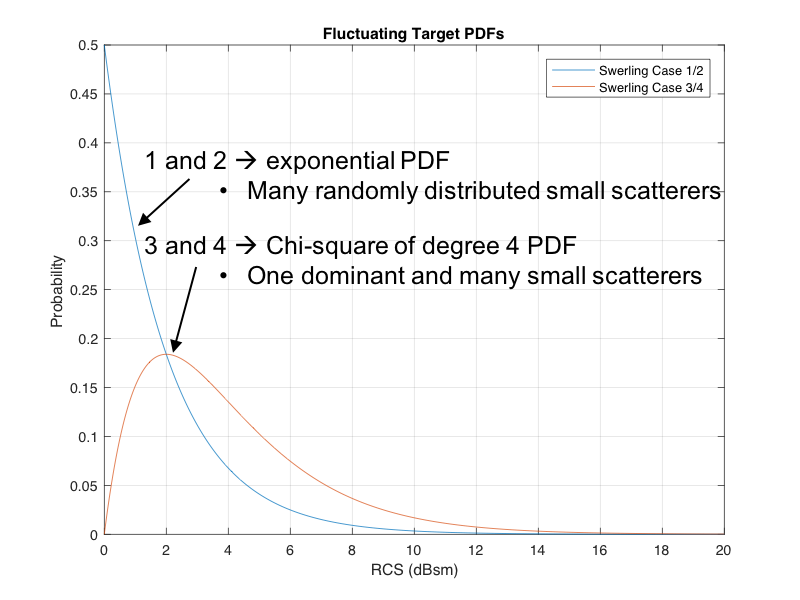
\includegraphics[width=4in]{../media/multistatic/swerling_pdfs.png}
  \end{center}
  \renewcommand{\baselinestretch}{1} \small\normalsize
  \begin{quote}
    \caption[Swerling Target Fluctuation Model PDFs]{Swerling Target Fluctuation Model PDFs\label{ms_fig:2}}
  \end{quote}
\end{figure}
\renewcommand{\baselinestretch}{2} \small\normalsize

The long decorrelation time covers the case where the target RCS can be considered constant over the time the RADAR performs a single scan and the short decorrelation time covers the case where the target RCS fluctuates on a pulse to pulse basis. Modern RADAR systems operate in frequency agile modes where the carrier frequency is changed each pulse, in which case the decorrelation time can be considered to be short. A fluctuating signal can have a significant effect on the $P_d$, as seen in Figure \ref{ms_fig:3} which shows the $P_d$ as a function of Signal to Noise Ratio (SNR) for the nonfluctating case and each of the $4$ Swerling cases. In this figure, we can see that using the wrong PDF can result in significantly overestimating the $P_d$.
\begin{figure}[H]
  \begin{center}
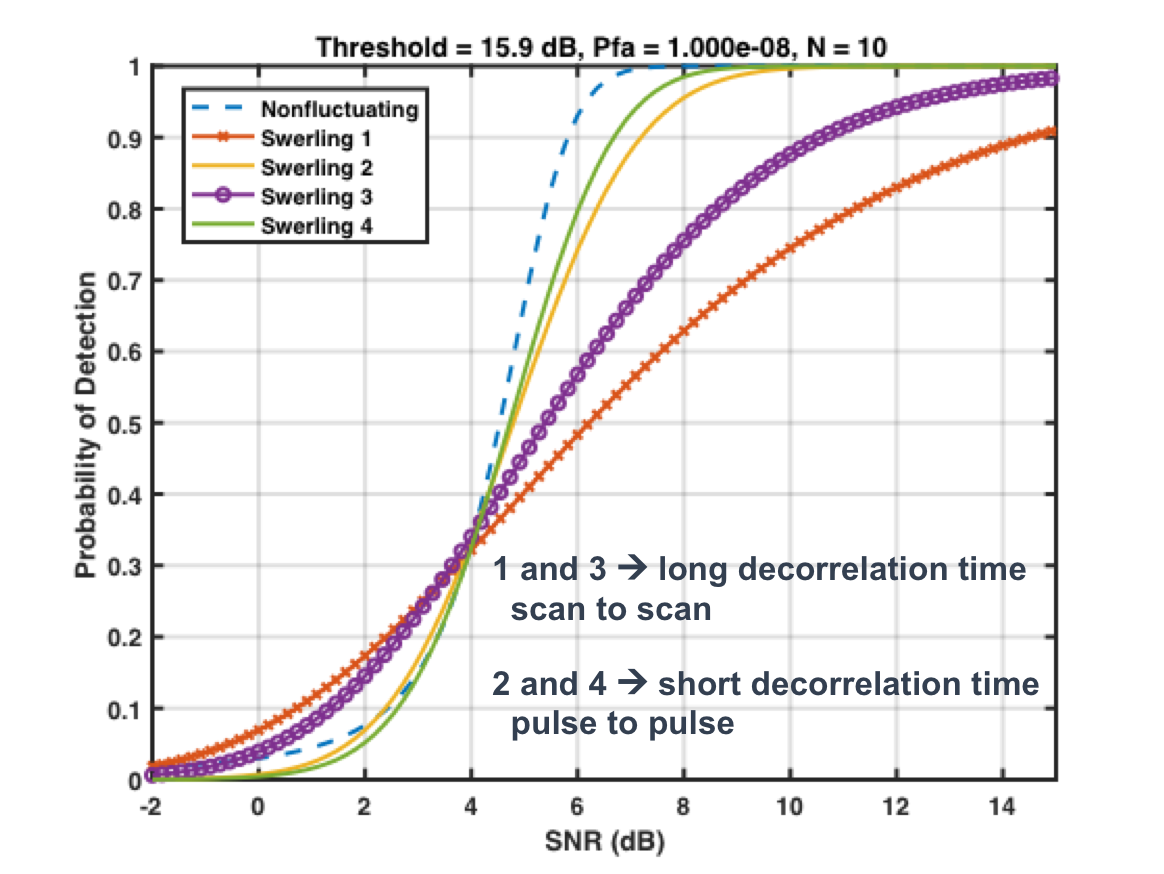
\includegraphics[width=4in]{../media/multistatic/swerling_pd.png}
  \end{center}
  \renewcommand{\baselinestretch}{1} \small\normalsize
  \begin{quote}
    \caption[Swerling Target Fluctuation Model Probability of Detection]{Swerling Target Fluctuation Model Probability of Detection\label{ms_fig:3}}
  \end{quote}
\end{figure}
\renewcommand{\baselinestretch}{2} \small\normalsize

Figure \ref{ms_fig:3} also shows that the $P_d$ is higher with a dominant scatterer than with a collection of uniform scatterers and that it is higher for a short decorrelation time than a long decorrelation time. We can force the decorrelation time to be short by operating in a frequency agile mode, but we generally have no control over the target configuration.